\chapter{Migliorare la Generalizzazione}

La \textbf{generalizzazione} rappresenta il cuore del Machine Learning: un modello non deve semplicemente memorizzare i dati del training set, ma dev’essere in grado di effettuare previsioni accurate anche su esempi mai visti prima. Per questo motivo, i dataset sono solitamente suddivisi in training set e test set: quest’ultimo non viene mostrato al modello durante l’addestramento, ma serve a valutare la capacità di generalizzazione. Nel contesto del Deep Learning, la questione diventa ancora più delicata: i modelli hanno un’elevata capacità espressiva e possono facilmente adattarsi in modo eccessivo ai dati di addestramento, fenomeno noto come \textbf{Overfitting}.

\section{Overfitting}

L’\textbf{Overfitting} si verifica quando un modello si adatta troppo ai dati di training, arrivando a modellare anche rumore e irregolarità accidentali, spesso dovute a errori di campionamento. In questi casi, il modello perde la capacità di distinguere tra regolarità significative e dettagli irrilevanti. Questo accade in particolare con modelli molto flessibili, che hanno una capacità sufficiente per apprendere qualsiasi cosa, incluse le fluttuazioni casuali dei dati.

\begin{quote}
\emph{"Se un modello è abbastanza potente da spiegare tutto, finirà per spiegare anche ciò che non è rilevante."}
\end{quote}

\begin{Osservazione}
    Un bel modo per visualizzare il fenomeno dell'overfitting, è immaginare una persona che si veste con delle taglie di vestiti differenti. Quando un vestito risulta essere troppo aderente parleremo di overfitting, quando un vestito è troppo largo parleremo di underfitting, mentre quando un capo è della giusta misura non avremo alcuna di queste problematiche.
\end{Osservazione}

\subsection{Prevenire l’Overfitting}

Per prevenire l’Overfitting, si possono adottare tre strategie principali, oltre a quelle già viste nel corso base di Machine Learning:

\begin{itemize}
\item \textbf{Espandere il dataset}, ovvero ottenere più dati. È la soluzione più efficace, ma spesso difficile da realizzare nella pratica;
\item \textbf{Utilizzare modelli con capacità adeguata}, evitando reti troppo semplici (Underfitting) o troppo complesse (Overfitting);
\item \textbf{Combinare più modelli} (ensemble), utilizzando architetture diverse o addestramenti su sottoinsiemi dei dati.
\end{itemize}

L’espansione del dataset aiuta a ridurre il rumore e aumenta la significatività statistica. I modelli troppo complessi rischiano l’Overfitting, mentre quelli troppo semplici non riescono a catturare la struttura dei dati (Underfitting). Infine, l’ensembling permette di mediare tra i diversi comportamenti, bilanciando bias e varianza, questa possibilità viene effettuato utilizzando tecniche di \textit{bagging} e \textit{boosting}, su cui ci soffermeremo più avanti.

\section{Limitare la capacità di un modello}

La capacità di un modello può essere controllata in diversi modi:

\begin{itemize}
\item \textbf{Architettura}: definizione del numero di layer e neuroni;
\item \textbf{Early Stopping}: interrompere l’addestramento prima che inizi l’Overfitting;
\item \textbf{Weight Decay}: aggiungere una penalizzazione ai pesi grandi tramite regolarizzazione L1 o L2;
\item \textbf{Noise Injection}: aggiungere rumore agli input o alle attivazioni per migliorare la robustezza.
\end{itemize}

Tutte queste tecniche mirano a ridurre la complessità effettiva del modello, favorendo una maggiore capacità di generalizzazione.

\subsection{Early Stopping}

L’\textbf{Early Stopping} è una tecnica che interrompe l’addestramento nel momento in cui il modello inizia a sovra-adattarsi ai dati. Nelle prime fasi, i pesi sono piccoli e i neuroni operano nella regione lineare; col progredire dell’allenamento, i pesi aumentano, i neuroni entrano nella regione non lineare e il modello diventa più potente, rischiando però l’Overfitting. Fermare l’allenamento nel momento opportuno consente di mantenere una buona capacità predittiva. È pratica comune utilizzare un \textbf{Validation Set} per monitorare l’andamento dell’errore e decidere quando arrestare l’addestramento.

\subsection{Weight Decay}

La regolarizzazione L2 introduce un termine additivo nella funzione di costo per penalizzare i pesi grandi:

\begin{equation}
J(\theta) = \mathcal{L}(\theta) + \lambda \sum_i \theta_i^2
\end{equation}

Questo termine forza i pesi a rimanere piccoli, evitando soluzioni troppo complesse. Il parametro $\lambda$ controlla l’intensità della penalizzazione:

\begin{itemize}
\item $\lambda$ troppo grande $\Rightarrow$ Underfitting;
\item $\lambda$ troppo piccolo $\Rightarrow$ rischio di Overfitting.
\end{itemize}

La regolarizzazione L1 $ (\sum_i |\theta_i|)$ è un’alternativa che induce \textbf{sparsità}, cioè tende a portare molti pesi a zero, dunque adoperando una sorta di selezione delle features.

\subsection{Noise Injection}

Aggiungere rumore ai dati d’ingresso o ai pesi agisce come regolarizzatore. Ad esempio aggiungendo un \textbf{rumore Gaussiano}:
\[
x_t^{(noisy)} = x_t + \mathcal{N}(0, \sigma^2)
\]
Il rumore, amplificato dai pesi, penalizza indirettamente pesi grandi. L’effetto è simile al weight decay: il modello diventa più robusto e meno dipendente da feature specifiche.

\section{Ensembling}

Combinare più modelli, o \textbf{Ensembling}, è una tecnica potente per migliorare la generalizzazione. L’errore totale può essere scomposto in:
\[
\text{Errore totale} = \text{Bias}^2 + \text{Varianza} + \text{Rumore}
\]

\begin{itemize}
  \item Modelli semplici: alto bias, bassa varianza;
  \item Modelli complessi: basso bias, alta varianza;
  \item Ensemble: riduce la varianza mantenendo basso il bias.
\end{itemize}

La media tra modelli riduce le fluttuazioni casuali. Anche se un singolo modello può occasionalmente performare meglio, in media l’ensemble è più stabile e generalizzabile. La diversità tra i modelli è cruciale.

\subsection{Sfruttare la diversità}

Un ensemble efficace richiede modelli diversi. Possiamo ottenerla:
\begin{itemize}
  \item Convergenza verso minimi locali diversi;
  \item Modelli eterogenei (es. SVM, alberi, reti);
  \item Architetture diverse: layer, neuroni, attivazioni, regolarizzazioni, ottimizzatori.
\end{itemize}

Modelli troppo simili generano ensemble inefficaci. Tecniche comuni per ottenere diversità:
\begin{itemize}
  \item \textbf{Bagging}: campionamento con rimpiazzo, riduce varianza;
  \item \textbf{Boosting}: sequenze di modelli deboli, riduce bias.
\end{itemize}

\begin{figure}
    \centering
    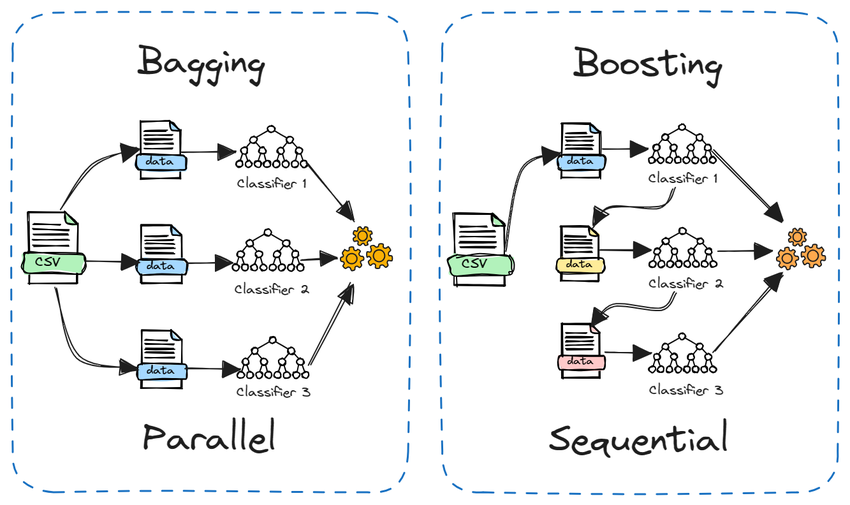
\includegraphics[width=0.85\textwidth]{figure/BagBoost.png}
    \caption{Rappresentazione dell’Ensemble tramite Bagging (sinistra) e Boosting (destra).}
    \label{fig:bagBoost}
\end{figure}

\subsubsection{Mixture of Models}
\[
P(y\,|\,x) = \sum_i \alpha_i P_i(y\,|\,x)
\]

\subsubsection{Product of Models}
\[
P(y\,|\,x) \propto \prod_i P_i(y\,|\,x)
\]

\section{Dropout}

Il \textbf{Dropout} è una tecnica di regolarizzazione che disattiva casualmente neuroni durante l’addestramento, simulando un ensemble di reti più piccole che condividono i pesi. Ogni forward pass attiva una sottorete diversa, riducendo la dipendenza da co-attivazioni specifiche. Con \( H \) neuroni, si campionano \( 2^H \) reti. I pesi sono condivisi, quindi ogni sottorete è fortemente regolarizzata. Il dropout riduce gli adattamenti complessi tra neuroni e rafforza la robustezza.

\begin{figure}
    \centering
    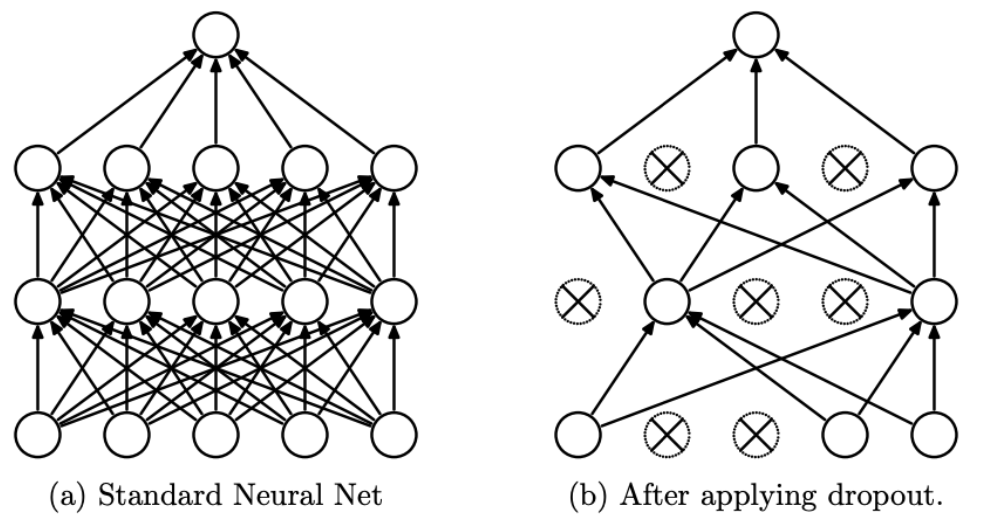
\includegraphics[width=0.85\textwidth]{figure/Dropout.png}
    \label{fig:dropout}
\end{figure}

\begin{itemize}
    \item Campionare più architetture e fare media geometrica (lento);
    \item Usare tutti i neuroni ma scalare i pesi in uscita con \( p \) (efficiente).
\end{itemize}

Se \( p = 0.5 \), allora a test-time:
\[
\theta_\text{test} = 0.5 \cdot \theta_\text{train}
\]
\marginpar{\href{https://www.cs.toronto.edu/~rsalakhu/papers/srivastava14a.pdf}{Srivastava et al. (2014)~\cite{srivastava2014dropout}}}
Come è stato formalizzato grazie ad alcuni ricercatori, questa procedura approssima la media dei modelli campionati. Il dropout può essere applicato anche agli input, con probabilità di disattivazione più bassa (es. $p=0.8$).

\subsubsection{Vantaggi}
\begin{itemize}
\item I neuroni non sanno con chi collaboreranno;
\item Devono produrre feature utili da sole;
\item Viene evitata la formazione di co-adattamenti complessi e fragili.
\end{itemize}

Il Dropout non è solo una forma di regolarizzazione numerica, ma impone una \emph{robustezza strutturale}, in cui ogni neurone dev’essere \textbf{indipendentemente utile}.

\begin{table}[h]
    \centering
    \caption{Strategie per migliorare la generalizzazione nei modelli di Deep Learning}
    \begin{adjustbox}{width=\textwidth}
    \begin{tabular}{@{}l|l@{}}
    \toprule
    \textbf{Tecnica} & \textbf{Descrizione} \\
    \midrule
    \textbf{Aumento dei dati} & Espandere il dataset con esempi reali o sintetici \\
    \textbf{Architettura adeguata} & Scegliere la capacità del modello con attenzione \\
    \textbf{Early Stopping} & Interrompere l’addestramento in tempo utile \\
    \textbf{Weight Decay} & Penalizzare pesi grandi nella funzione di loss \\
    \textbf{Noise Injection} & Aggiungere rumore a input o attivazioni \\
    \textbf{Ensemble} & Media di modelli diversi per ridurre la varianza \\
    \textbf{Bagging} & Campionamento con rimpiazzo per ensemble \\
    \textbf{Boosting} & Addestramento sequenziale di modelli deboli \\
    \textbf{Dropout} & Spegnere neuroni casualmente evitando adattamenti \\
    \bottomrule
    \end{tabular}
    \end{adjustbox}
\end{table}
